\documentclass{standalone}
\usepackage{tikz}
\usetikzlibrary{patterns, positioning}
\usepackage[sfdefault]{ClearSans} %% option 'sfdefault' activates Clear Sans as the default text font
\usepackage[T1]{fontenc}

\begin{document}
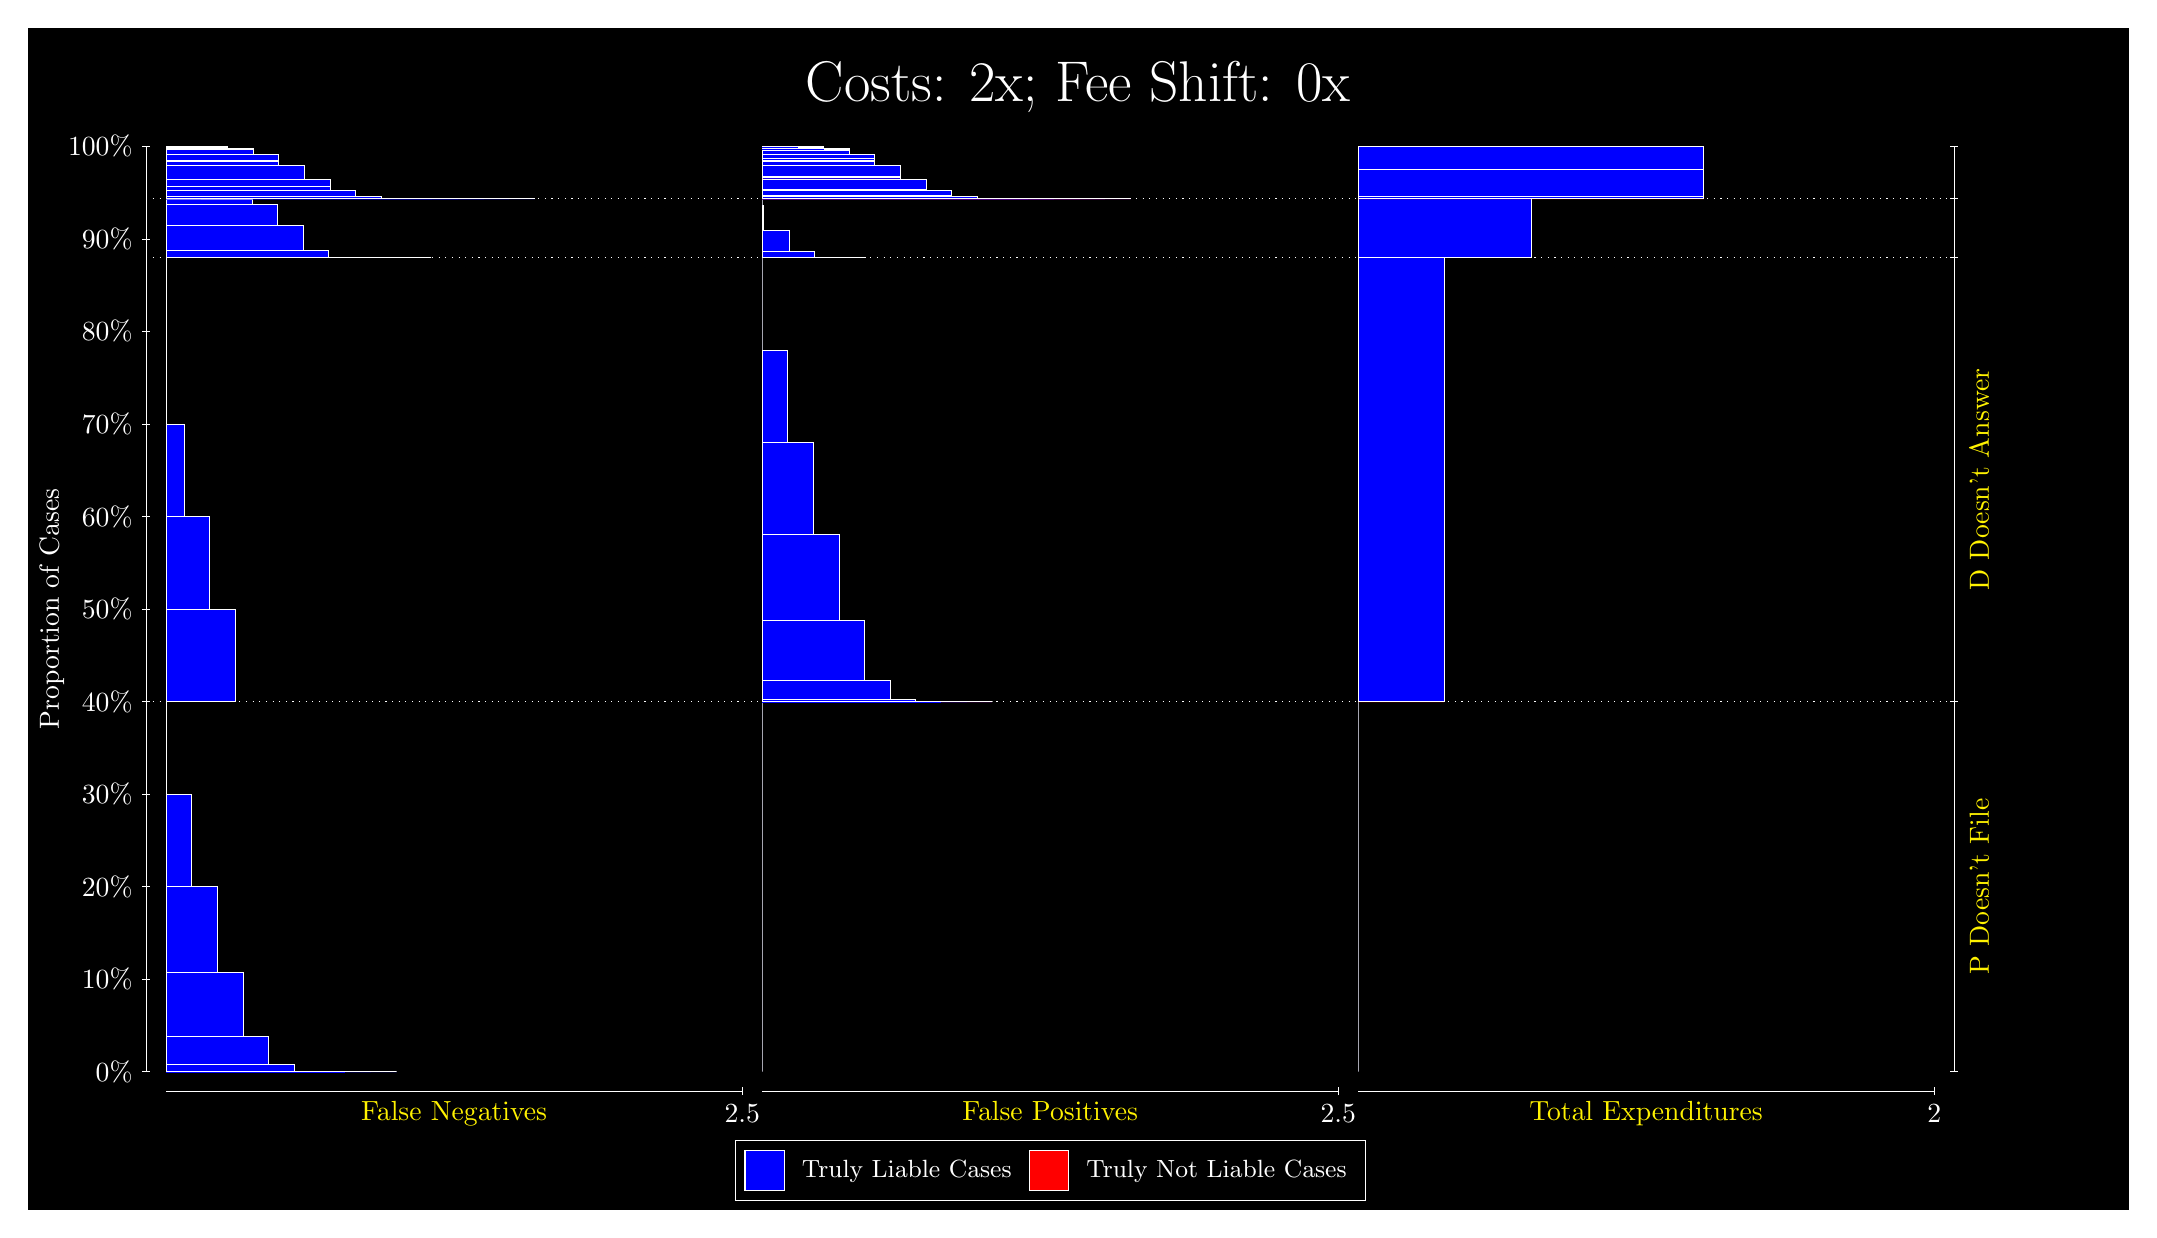
\begin{tikzpicture}
\draw[fill=black] (0,0) rectangle (26.667,15);
\draw[text=white] (0,13.5) rectangle (26.667,15) node[midway] {\huge Costs: 2x; Fee Shift: 0x};
\draw[white, very thin] (1.5,1.75) -- (1.5,13.5);
\node[rotate=90, text=white, anchor=center] at (0.3, 7.625) {Proportion of Cases};
\draw[white, very thin] (1.45,1.75) -- (1.55,1.75);
\node[text=white, anchor=east] at (1.45, 1.75) {0\%};
\draw[white, very thin] (1.45,2.925) -- (1.55,2.925);
\node[text=white, anchor=east] at (1.45, 2.925) {10\%};
\draw[white, very thin] (1.45,4.1) -- (1.55,4.1);
\node[text=white, anchor=east] at (1.45, 4.1) {20\%};
\draw[white, very thin] (1.45,5.275) -- (1.55,5.275);
\node[text=white, anchor=east] at (1.45, 5.275) {30\%};
\draw[white, very thin] (1.45,6.45) -- (1.55,6.45);
\node[text=white, anchor=east] at (1.45, 6.45) {40\%};
\draw[white, very thin] (1.45,7.625) -- (1.55,7.625);
\node[text=white, anchor=east] at (1.45, 7.625) {50\%};
\draw[white, very thin] (1.45,8.8) -- (1.55,8.8);
\node[text=white, anchor=east] at (1.45, 8.8) {60\%};
\draw[white, very thin] (1.45,9.975) -- (1.55,9.975);
\node[text=white, anchor=east] at (1.45, 9.975) {70\%};
\draw[white, very thin] (1.45,11.15) -- (1.55,11.15);
\node[text=white, anchor=east] at (1.45, 11.15) {80\%};
\draw[white, very thin] (1.45,12.325) -- (1.55,12.325);
\node[text=white, anchor=east] at (1.45, 12.325) {90\%};
\draw[white, very thin] (1.45,13.5) -- (1.55,13.5);
\node[text=white, anchor=east] at (1.45, 13.5) {100\%};

\draw[white, very thin] (24.457,1.75) -- (24.457,13.5);
\draw[white, very thin] (24.407,1.75) -- (24.507,1.75);
\node[anchor=west] at (24.407, 1.75) {};
\draw[white, very thin] (24.407,6.4488) -- (24.507,6.4488);
\node[anchor=west] at (24.407, 6.4488) {};
\draw[white, very thin] (24.407,12.089) -- (24.507,12.089);
\node[anchor=west] at (24.407, 12.089) {};
\draw[white, very thin] (24.407,12.837) -- (24.507,12.837);
\node[anchor=west] at (24.407, 12.837) {};
\draw[white, very thin] (24.407,13.5) -- (24.507,13.5);
\node[anchor=west] at (24.407, 13.5) {};

\draw[white, very thin, fill=blue] (1.75,1.75) rectangle (4.6775,1.75);
\draw[white, very thin, fill=blue] (1.75,1.75) rectangle (4.3523,1.75);
\draw[white, very thin, fill=blue] (1.75,1.75) rectangle (4.027,1.7503);
\draw[white, very thin, fill=blue] (1.75,1.7503) rectangle (3.7017,1.7576);
\draw[white, very thin, fill=blue] (1.75,1.7576) rectangle (3.3764,1.8361);
\draw[white, very thin, fill=blue] (1.75,1.8361) rectangle (3.0511,2.1986);
\draw[white, very thin, fill=blue] (1.75,2.1986) rectangle (2.7258,3.011);
\draw[white, very thin, fill=blue] (1.75,3.011) rectangle (2.4006,4.107);
\draw[white, very thin, fill=blue] (1.75,4.107) rectangle (2.0753,5.2742);
\draw[white, very thin, fill=red] (1.75,5.2742) rectangle (1.75,5.2742);
\draw[white, very thin, fill=blue] (1.75,5.2742) rectangle (1.75,6.4488);
\draw[white, very thin, fill=blue] (1.75,6.4488) rectangle (2.6283,7.6238);
\draw[white, very thin, fill=blue] (1.75,7.6238) rectangle (2.303,8.7986);
\draw[white, very thin, fill=blue] (1.75,8.7986) rectangle (1.9777,9.9659);
\draw[white, very thin, fill=red] (1.75,9.9659) rectangle (1.75,9.9659);
\draw[white, very thin, fill=blue] (1.75,9.9659) rectangle (1.75,12.089);
\draw[white, very thin, fill=blue] (1.75,12.089) rectangle (5.1167,12.089);
\draw[white, very thin, fill=blue] (1.75,12.089) rectangle (4.7914,12.089);
\draw[white, very thin, fill=blue] (1.75,12.089) rectangle (4.4661,12.089);
\draw[white, very thin, fill=blue] (1.75,12.089) rectangle (4.1408,12.094);
\draw[white, very thin, fill=blue] (1.75,12.094) rectangle (3.8155,12.182);
\draw[white, very thin, fill=blue] (1.75,12.182) rectangle (3.4903,12.493);
\draw[white, very thin, fill=blue] (1.75,12.493) rectangle (3.165,12.758);
\draw[white, very thin, fill=blue] (1.75,12.758) rectangle (2.8397,12.829);
\draw[white, very thin, fill=blue] (1.75,12.829) rectangle (2.5144,12.837);
\draw[white, very thin, fill=blue] (1.75,12.837) rectangle (2.1891,12.837);
\draw[white, very thin, fill=red] (1.75,12.837) rectangle (1.75,12.837);
\draw[white, very thin, fill=blue] (1.75,12.837) rectangle (6.4341,12.837);
\draw[white, very thin, fill=blue] (1.75,12.837) rectangle (6.1088,12.837);
\draw[white, very thin, fill=blue] (1.75,12.837) rectangle (5.7835,12.837);
\draw[white, very thin, fill=blue] (1.75,12.837) rectangle (5.4582,12.837);
\draw[white, very thin, fill=blue] (1.75,12.837) rectangle (5.1329,12.837);
\draw[white, very thin, fill=blue] (1.75,12.837) rectangle (4.8077,12.84);
\draw[white, very thin, fill=blue] (1.75,12.84) rectangle (4.8077,12.842);
\draw[white, very thin, fill=blue] (1.75,12.842) rectangle (4.4824,12.867);
\draw[white, very thin, fill=blue] (1.75,12.867) rectangle (4.4824,12.867);
\draw[white, very thin, fill=blue] (1.75,12.867) rectangle (4.1571,12.941);
\draw[white, very thin, fill=blue] (1.75,12.941) rectangle (3.8318,12.996);
\draw[white, very thin, fill=blue] (1.75,12.996) rectangle (3.8318,13.082);
\draw[white, very thin, fill=blue] (1.75,13.082) rectangle (3.5065,13.255);
\draw[white, very thin, fill=blue] (1.75,13.255) rectangle (3.1812,13.31);
\draw[white, very thin, fill=blue] (1.75,13.31) rectangle (3.1812,13.327);
\draw[white, very thin, fill=blue] (1.75,13.327) rectangle (3.1812,13.396);
\draw[white, very thin, fill=blue] (1.75,13.396) rectangle (2.856,13.461);
\draw[white, very thin, fill=blue] (1.75,13.461) rectangle (2.856,13.47);
\draw[white, very thin, fill=blue] (1.75,13.47) rectangle (2.5307,13.479);
\draw[white, very thin, fill=blue] (1.75,13.479) rectangle (2.5307,13.482);
\draw[white, very thin, fill=blue] (1.75,13.482) rectangle (2.5307,13.495);
\draw[white, very thin, fill=blue] (1.75,13.495) rectangle (2.2054,13.499);
\draw[white, very thin, fill=blue] (1.75,13.499) rectangle (2.2054,13.5);
\draw[white, very thin, fill=blue] (1.75,13.5) rectangle (1.8801,13.5);
\draw[white, very thin, fill=blue] (1.75,13.5) rectangle (1.8801,13.5);
\draw[white, very thin, fill=red] (1.75,13.5) rectangle (1.75,13.5);
\draw[white, very thin, fill=blue] (1.75,13.5) rectangle (1.75,13.5);
\draw[white, very thin, fill=red] (9.3189,1.75) rectangle (9.3189,1.75);
\draw[white, very thin, fill=blue] (9.3189,1.75) rectangle (9.3189,6.4488);
\draw[white, very thin, fill=red] (9.3189,6.4488) rectangle (12.246,6.4488);
\draw[white, very thin, fill=blue] (9.3189,6.4488) rectangle (12.246,6.4488);
\draw[white, very thin, fill=blue] (9.3189,6.4488) rectangle (11.921,6.4488);
\draw[white, very thin, fill=blue] (9.3189,6.4488) rectangle (11.596,6.4493);
\draw[white, very thin, fill=blue] (9.3189,6.4493) rectangle (11.271,6.4736);
\draw[white, very thin, fill=blue] (9.3189,6.4736) rectangle (10.945,6.7242);
\draw[white, very thin, fill=blue] (9.3189,6.7242) rectangle (10.62,7.4824);
\draw[white, very thin, fill=blue] (9.3189,7.4824) rectangle (10.295,8.5721);
\draw[white, very thin, fill=blue] (9.3189,8.5721) rectangle (9.9694,9.7395);
\draw[white, very thin, fill=blue] (9.3189,9.7395) rectangle (9.6442,10.914);
\draw[white, very thin, fill=blue] (9.3189,10.914) rectangle (9.3189,12.089);
\draw[white, very thin, fill=red] (9.3189,12.089) rectangle (10.636,12.089);
\draw[white, very thin, fill=blue] (9.3189,12.089) rectangle (10.636,12.09);
\draw[white, very thin, fill=blue] (9.3189,12.09) rectangle (10.311,12.097);
\draw[white, very thin, fill=blue] (9.3189,12.097) rectangle (9.9857,12.168);
\draw[white, very thin, fill=blue] (9.3189,12.168) rectangle (9.6604,12.433);
\draw[white, very thin, fill=blue] (9.3189,12.433) rectangle (9.3351,12.745);
\draw[white, very thin, fill=blue] (9.3189,12.745) rectangle (9.3189,12.837);
\draw[white, very thin, fill=red] (9.3189,12.837) rectangle (14.003,12.837);
\draw[white, very thin, fill=blue] (9.3189,12.837) rectangle (14.003,12.837);
\draw[white, very thin, fill=red] (9.3189,12.837) rectangle (13.678,12.837);
\draw[white, very thin, fill=blue] (9.3189,12.837) rectangle (13.678,12.837);
\draw[white, very thin, fill=red] (9.3189,12.837) rectangle (13.352,12.837);
\draw[white, very thin, fill=blue] (9.3189,12.837) rectangle (13.352,12.837);
\draw[white, very thin, fill=blue] (9.3189,12.837) rectangle (13.027,12.837);
\draw[white, very thin, fill=red] (9.3189,12.837) rectangle (13.027,12.837);
\draw[white, very thin, fill=blue] (9.3189,12.837) rectangle (13.027,12.837);
\draw[white, very thin, fill=blue] (9.3189,12.837) rectangle (12.702,12.837);
\draw[white, very thin, fill=red] (9.3189,12.837) rectangle (12.702,12.837);
\draw[white, very thin, fill=blue] (9.3189,12.837) rectangle (12.702,12.837);
\draw[white, very thin, fill=blue] (9.3189,12.837) rectangle (12.377,12.842);
\draw[white, very thin, fill=red] (9.3189,12.842) rectangle (12.377,12.842);
\draw[white, very thin, fill=blue] (9.3189,12.842) rectangle (12.377,12.842);
\draw[white, very thin, fill=blue] (9.3189,12.842) rectangle (12.051,12.845);
\draw[white, very thin, fill=red] (9.3189,12.845) rectangle (12.051,12.845);
\draw[white, very thin, fill=blue] (9.3189,12.845) rectangle (12.051,12.867);
\draw[white, very thin, fill=blue] (9.3189,12.867) rectangle (12.051,12.867);
\draw[white, very thin, fill=blue] (9.3189,12.867) rectangle (12.051,12.867);
\draw[white, very thin, fill=blue] (9.3189,12.867) rectangle (11.726,12.876);
\draw[white, very thin, fill=red] (9.3189,12.876) rectangle (11.726,12.876);
\draw[white, very thin, fill=blue] (9.3189,12.876) rectangle (11.726,12.94);
\draw[white, very thin, fill=blue] (9.3189,12.94) rectangle (11.726,12.941);
\draw[white, very thin, fill=blue] (9.3189,12.941) rectangle (11.401,12.941);
\draw[white, very thin, fill=blue] (9.3189,12.941) rectangle (11.401,12.96);
\draw[white, very thin, fill=red] (9.3189,12.96) rectangle (11.401,12.96);
\draw[white, very thin, fill=blue] (9.3189,12.96) rectangle (11.401,13.082);
\draw[white, very thin, fill=blue] (9.3189,13.082) rectangle (11.075,13.101);
\draw[white, very thin, fill=red] (9.3189,13.101) rectangle (11.075,13.101);
\draw[white, very thin, fill=blue] (9.3189,13.101) rectangle (11.075,13.124);
\draw[white, very thin, fill=blue] (9.3189,13.124) rectangle (11.075,13.255);
\draw[white, very thin, fill=blue] (9.3189,13.255) rectangle (10.75,13.308);
\draw[white, very thin, fill=blue] (9.3189,13.308) rectangle (10.75,13.324);
\draw[white, very thin, fill=blue] (9.3189,13.324) rectangle (10.75,13.343);
\draw[white, very thin, fill=blue] (9.3189,13.343) rectangle (10.75,13.396);
\draw[white, very thin, fill=blue] (9.3189,13.396) rectangle (10.425,13.452);
\draw[white, very thin, fill=blue] (9.3189,13.452) rectangle (10.425,13.461);
\draw[white, very thin, fill=blue] (9.3189,13.461) rectangle (10.425,13.47);
\draw[white, very thin, fill=blue] (9.3189,13.47) rectangle (10.1,13.472);
\draw[white, very thin, fill=blue] (9.3189,13.472) rectangle (10.1,13.475);
\draw[white, very thin, fill=blue] (9.3189,13.475) rectangle (10.1,13.494);
\draw[white, very thin, fill=blue] (9.3189,13.494) rectangle (10.1,13.495);
\draw[white, very thin, fill=blue] (9.3189,13.495) rectangle (9.7743,13.497);
\draw[white, very thin, fill=blue] (9.3189,13.497) rectangle (9.7743,13.5);
\draw[white, very thin, fill=blue] (9.3189,13.5) rectangle (9.449,13.5);
\draw[white, very thin, fill=blue] (9.3189,13.5) rectangle (9.449,13.5);
\draw[white, very thin, fill=blue] (9.3189,13.5) rectangle (9.449,13.5);
\draw[white, very thin, fill=blue] (9.3189,13.5) rectangle (9.3189,13.5);
\draw[white, very thin, fill=red] (16.888,1.75) rectangle (16.888,1.75);
\draw[white, very thin, fill=blue] (16.888,1.75) rectangle (16.888,6.4488);
\draw[white, very thin, fill=red] (16.888,6.4488) rectangle (17.986,6.4488);
\draw[white, very thin, fill=blue] (16.888,6.4488) rectangle (17.986,12.089);
\draw[white, very thin, fill=red] (16.888,12.089) rectangle (19.083,12.089);
\draw[white, very thin, fill=blue] (16.888,12.089) rectangle (19.083,12.837);
\draw[white, very thin, fill=red] (16.888,12.837) rectangle (21.279,12.837);
\draw[white, very thin, fill=blue] (16.888,12.837) rectangle (21.279,12.865);
\draw[white, very thin, fill=red] (16.888,12.865) rectangle (21.279,12.865);
\draw[white, very thin, fill=blue] (16.888,12.865) rectangle (21.279,13.213);
\draw[white, very thin, fill=red] (16.888,13.213) rectangle (21.279,13.213);
\draw[white, very thin, fill=blue] (16.888,13.213) rectangle (21.279,13.5);
\draw[white, dotted] (1.5,6.4488) -- (24.457,6.4488);
\draw[white, dotted] (1.5,12.089) -- (24.457,12.089);
\draw[white, dotted] (1.5,12.837) -- (24.457,12.837);
\draw[white, very thin] (1.75,1.5) -- (9.0689,1.5);
\node[text=yellow, anchor=north] at (5.4094, 1.5) {False Negatives};
\draw[white, very thin] (9.0689,1.45) -- (9.0689,1.55);
\node[text=white, anchor=north] at (9.0689, 1.45) {2.5};

\draw[white, very thin] (9.3189,1.5) -- (16.638,1.5);
\node[text=yellow, anchor=north] at (12.978, 1.5) {False Positives};
\draw[white, very thin] (16.638,1.45) -- (16.638,1.55);
\node[text=white, anchor=north] at (16.638, 1.45) {2.5};

\draw[white, very thin] (16.888,1.5) -- (24.207,1.5);
\node[text=yellow, anchor=north] at (20.547, 1.5) {Total Expenditures};
\draw[white, very thin] (24.207,1.45) -- (24.207,1.55);
\node[text=white, anchor=north] at (24.207, 1.45) {2};

\node[text=yellow, centered, rotate=90] at (24.777, 4.0994) {P Doesn't File};
\node[text=yellow, centered, rotate=90] at (24.777, 9.269) {D Doesn't Answer};



\draw (12.978300999999998,1.5) node[draw=none] (baseCoordinate) {};
\begin{scope}[align=center]
        \matrix[scale=0.5, draw=white, below=0.5cm of baseCoordinate, nodes={draw}, column sep=0.1cm]{
            \node[rectangle, draw, minimum width=0.5cm, minimum height=0.5cm, fill=blue] {}; &
            \node[draw=none, font=\small, text=white] (B) {Truly Liable Cases}; &
            \node[rectangle, draw, minimum width=0.5cm, minimum height=0.5cm, fill=red] {}; &
            \node[draw=none, font=\small, text=white] (B) {Truly Not Liable Cases}; \\
            };
\end{scope}

\end{tikzpicture}
\end{document}